\section{PipeWire}

\subsection{Introduction}

\begin{frame}{Introduction}
  \begin{itemize}
  \item A realtime multimedia data graph
  \item Works across processes
  \item Why?
    \begin{itemize}
    \item Sharing of devices across processes
    \item Dynamic routing at runtime
    \item Implements format negociation \& conversion
    \item Modular audio processing, spread across Linux processes
    \item Low overhead: shared memory for data and no roundtrip to daemon
    \end{itemize}
  \item Same abstraction layer (alternatives)
    \begin{itemize}
    \item \href{https://www.freedesktop.org/wiki/Software/PulseAudio/}{PulseAudio}
    \item \href{https://jackaudio.org/}{JACK Audio Connection Kit}
    \end{itemize}
  \item Technical stack: C (\code{gnu11}), Meson \& Ninja
  \end{itemize}
\end{frame}



\begin{frame}[fragile]{Concepts — objects}

  \begin{itemize}
  \item The graph state representation is a list of objects.
  \item That object list is handled by the \code{Core} object, hosted
    by the PipeWire daemon.
  \item Each connected process is represented by a \code{Client} object.
  \end{itemize}

  \begin{columns}

    \column{0.5\textwidth}
      Example with \code{pw-play audio.wav} and
      \code{pw-record --target pw-play rec.wav}:

      \begin{block}{}
        \fontsize{8}{8}\selectfont
          \begin{minted}{text}
$ pw-cli ls Core
    id 0, type PipeWire:Interface:Core/4
        object.serial = "0"
        core.name = "pipewire-0"
          \end{minted}
        \end{block}

    \column{0.5\textwidth}
      \begin{block}{}
        \fontsize{8}{8}\selectfont
          \begin{minted}{text}
$ pw-cli ls Client
    id 35, type PipeWire:Interface:Client/3
        object.serial = "35"
        pipewire.sec.pid = "2718"
        application.name = "pipewire"
    id 129, type PipeWire:Interface:Client/3
        object.serial = "11608"
        pipewire.sec.pid = "466490"
        application.name = "pw-cli"
    id 145, type PipeWire:Interface:Client/3
        object.serial = "11572"
        pipewire.sec.pid = "465686"
        application.name = "pw-cat"
    id 168, type PipeWire:Interface:Client/3
        object.serial = "11593"
        pipewire.sec.pid = "466186"
        application.name = "pw-cat"
    ...
          \end{minted}
        \end{block}

  \end{columns}
\end{frame}



\begin{frame}{Concepts — nodes, ports \& links (1)}
  \begin{itemize}

  \item The graph itself is represented by the following object types:

    \begin{itemize}
    \item A \code{Node} processes samples
    \item A \code{Port} represents a node input or output
    \item A \code{Link} connects an output port with an input port
    \end{itemize}

  \end{itemize}

  \begin{center}
    \includegraphics[height=0.4\textheight]{slides/audio-pipewire/two-nodes.pdf}\\
  \end{center}
\end{frame}



\begin{frame}[fragile]{Concepts — nodes, ports \& links (2)}

  \begin{columns}

    \column{0.5\textwidth}
      \begin{block}{}
        \fontsize{8}{8}\selectfont
          \begin{minted}{text}
$ pw-cli ls Node
    id 137, type PipeWire:Interface:Node/3
        client.id = "145"
        node.name = "pw-play"
        media.class = "Stream/Output/Audio"
    id 111, type PipeWire:Interface:Node/3
        client.id = "168"
        node.name = "pw-record"
        media.class = "Stream/Input/Audio"
    ...

$ pw-cli ls Link
    id 119, type PipeWire:Interface:Link/3
        client.id = "33"
        link.output.port = "116"
        link.input.port = "139"
        link.output.node = "137"
        link.input.node = "111"
    id 97, type PipeWire:Interface:Link/3
        client.id = "33"
        link.output.port = "115"
        link.input.port = "117"
        link.output.node = "137"
        link.input.node = "111"
    ...
          \end{minted}
        \end{block}


    \column{0.5\textwidth}
      \begin{block}{}
        \fontsize{8}{8}\selectfont
          \begin{minted}{text}
$ pw-cli ls Port
    id 116, type PipeWire:Interface:Port/3
        format.dsp = "32 bit float mono audio"
        node.id = "137"
        audio.channel = "FL"
        port.alias = "pw-play:output_FL"
    id 115, type PipeWire:Interface:Port/3
        format.dsp = "32 bit float mono audio"
        node.id = "137"
        audio.channel = "FR"
        port.alias = "pw-play:output_FR"
    id 139, type PipeWire:Interface:Port/3
        format.dsp = "32 bit float mono audio"
        node.id = "111"
        audio.channel = "FL"
        port.alias = "pw-record:input_FL"
    id 117, type PipeWire:Interface:Port/3
        format.dsp = "32 bit float mono audio"
        node.id = "111"
        audio.channel = "FR"
        port.alias = "pw-record:input_FR"
    ...
          \end{minted}
        \end{block}

  \end{columns}
\end{frame}



\begin{frame}[fragile]{Concepts — object properties and params}
  \begin{columns}

    \column{0.45\textwidth}
      \begin{itemize}
      \item Objects are defined by their ID and type.

      \item Objects also contain \textbf{properties}: a list of string
        key-value pairs. Those can only be modified by the client
        hosting the node.

      \item Some object types also contain \textbf{params}. Those might
        be configurable by other clients.

        \begin{itemize}
        \item They get used for format negociation \& conversion,
          volume control, etc.
        \end{itemize}
      \end{itemize}

    \column{0.55\textwidth}
    \begin{block}{}
      \fontsize{8}{8}\selectfont
        \begin{minted}{text}
$ pw-cli info 94
  type: PipeWire:Interface:Node/3
* properties:
*   application.name = "pw-play"
*   node.name = "pw-play"
*   media.type = "Audio"
*   media.category = "Playback"
*   media.role = "Music"
*   node.rate = "1/44100"
*   node.latency = "4410/44100"
*   node.autoconnect = "true"
*   node.want-driver = "true"
*   media.class = "Stream/Output/Audio"
*   factory.id = "8"
*   clock.quantum-limit = "8192"
*   library.name = "audioconvert/libspa-audioconvert"
*   client.id = "151"
*   object.id = "94"
*   object.serial = "2005"
*   ...
* params: (8)
*   3 (Spa:Enum:ParamId:EnumFormat) r-
*   2 (Spa:Enum:ParamId:Props) rw
*   4 (Spa:Enum:ParamId:Format) rw
*   ...
        \end{minted}
      \end{block}

  \end{columns}
\end{frame}



\begin{frame}{Concepts — devices}
  \begin{itemize}

  \item Another object type is \code{Device}. Those map to physical
    devices, to which are assigned one or more nodes. Device
    configuration is done via those objects.

  \item Providers can be alsa-lib, \href{http://www.bluez.org/}{BlueZ},
    \href{https://libcamera.org/}{libcamera},
    \href{https://en.wikipedia.org/wiki/Video4Linux}{V4L}, etc.

  \end{itemize}
\end{frame}



\begin{frame}{Concepts — graph execution logic (1)}
  \begin{itemize}

  \item PipeWire structures itself as multiple subgraphs. In each one
    of those, there is exactly one \textbf{driver} node, and zero or
    more \textbf{follower} nodes.

  \item The driver node is responsible for triggering the start of
    execution cycles, based on a timer or hardware interrupt for example.

  \item Each node keeps two counters:
    \begin{enumerate}
    \item \code{required}: the number of dependencies on other nodes;
    \item \code{pending}: how many remaining nodes need to be executed
      before it can run in this cycle. A value of zero means the node
      can be executed. Its reset value is \code{required}.
    \end{enumerate}

  \item Nodes also keep a list of nodes that depend on them (called
    targets); a node is responsible for decrementing its targets'
    \code{pending} counters and signal them using IPC.

  \item See \href{https://docs.pipewire.org/page_scheduling.html}{the
    documentation} for more details. The graph evaluation is
    implemented by \code{pw_context_recalc_graph()}.

  \end{itemize}
\end{frame}



\begin{frame}{Concepts — graph execution logic (2)}
  \begin{itemize}
  \item The driver node is picked based on the \code{priority.driver} property.
  \item A good default is to set higher priority to capture driver nodes.
  \end{itemize}

  \begin{center}
    \includegraphics[height=0.5\textheight]{slides/audio-pipewire/graph-execution.pdf}\\
  \end{center}
\end{frame}



\begin{frame}{Concepts — graph execution logic (3)}
  \begin{itemize}

  \item PipeWire clients and modules can create independent nodes
    rather than a single one with input and output ports. That allows
    having multiple subgraphs, each driven by a different driver node.

  \item \textbf{Virtual loopbacks} are such an example: they allow
    sending samples from a subgraph to another while still decoupling
    driver clocks.

  \end{itemize}

  \begin{center}
    \includegraphics[height=0.45\textheight]{slides/audio-pipewire/graph-execution2.pdf}\\
  \end{center}
\end{frame}



\begin{frame}{Concepts — graph execution logic (4)}
  \begin{itemize}

  \item The number of samples to be generated during a cycle is called
    \textbf{the quantum}.

  \item There are global settings for minimum and
    maximum, and nodes can request specific values for the subgraph
    they take part in.

  \item Nodes can also request for a locked quantum: that it does not
    get changed across recalculations of the graph. This gets used for
    applications that require fixed quantum (such as the JACK
    compatibility layer).

  \item The \textbf{rate} is similar: it can be different for each
    subgraph. The PipeWire config has a list of allowed rates.

  \end{itemize}
\end{frame}



\begin{frame}{Concepts — modules}
  \begin{itemize}

  \item Modules are libraries loaded by PipeWire clients to implement
    various features.

  \item Example modules:

    \begin{itemize}
    \item \code{module-rt}: requests realtime scheduling priority using
      \code{setpriority(2)} and \code{pthread_setschedparam(3)}.
    \item \code{module-loopback}: create two virtual loopback nodes.
    \item \code{module-protocol-native}: implements the communication
      between the daemon and clients.
    \item \code{module-profiler}: implements the profiling logic,
      attached to the daemon.
    \item etc.
    \end{itemize}

  \end{itemize}
\end{frame}



\begin{frame}{PipeWire communication protocols — IPC}
  \begin{itemize}

  \item \code{socket(AF_UNIX, SOCK_STREAM, 0)} for communication with
    the daemon process. The socket is named \code{pipewire-0} by
    default or \code{$PIPEWIRE_REMOTE}. Directory look-up order:
    \begin{enumerate}
    \item \code{$PIPEWIRE_RUNTIME_DIR}
    \item \code{$XDG_RUNTIME_DIR}
    \item \code{$USERPROFILE}
    \end{enumerate}
  \item \code{eventfd(2)} is the wakeup method.
  \item \code{memfd_create(2)} is used for sharing multimedia data
    across related clients (without data going through the daemon).
  \item PipeWire provides an event-loop implementation that relies
    upon \code{epoll(7)}. All clients use it. They also use
    \code{signalfd(2)} to handle signals.

  \end{itemize}
\end{frame}



\begin{frame}{PipeWire communication protocols — D-Bus optional dependency}
  \begin{itemize}

  \item Happens on the session bus
  \item Flatpak permission support through
    \href{https://docs.flatpak.org/en/latest/desktop-integration.html\#portals}{
    XDG Desktop Portal}, see \code{libpipewire-module-portal}
  \item Audio device reservation through the
    \href{https://git.0pointer.net/reserve.git/tree/reserve.txt}{
    org.freedesktop.ReserveDevice1}, see
    \code{libwireplumber-module-reserve-device}
  \item For Bluetooth support through
    \href{http://www.bluez.org/}{BlueZ}, see PipeWire's
    \code{libspa-bluez5}

  \end{itemize}
\end{frame}



\subsection{Configuration}



\begin{frame}{Configuration — location (1)}
  \begin{itemize}

  \item Each client locates and reads its configuration at startup.

  \item Those configuration files follow a PipeWire-specific format.

  \item Look-up order:
    \begin{enumerate}
    \item \code{$XDG_CONFIG_HOME/pipewire/}\\
      environment variable, often \code{~/.config/pipewire/} in distributions
    \item \code{$sysconfdir/pipewire/}\\
      compile-time variable, often \code{/etc/pipewire/}
    \item \code{$datadir/pipewire/}\\
      compile-time variable, often \code{/usr/share/pipewire/}
    \end{enumerate}

  \end{itemize}
\end{frame}



\begin{frame}{Configuration — location (2)}
  \begin{itemize}

  \item A client that loads a config file named \code{client-rt.conf}
    will load the first file named as such in the above folders, but
    will also load all config sections from:

    \begin{enumerate}
    \item \code{$datadir/pipewire/client-rt.conf.d/}
    \item \code{$sysconfdir/pipewire/client-rt.conf.d/}
    \item \code{$XDG_CONFIG_HOME/pipewire/client-rt.conf.d/}
    \end{enumerate}

  \end{itemize}
\end{frame}



\begin{frame}[fragile]{Configuration — sections (1)}

  \begin{itemize}
  \item \code{context.properties} configures the PipeWire instance.

  \item Most properties target the daemon
    (\code{default.clock.allowed-rates},
    \code{default.clock.max-quantum}, etc.) but some also apply to
    other clients (\code{log.level}, \code{mem.mlock-all}, etc.).
  \end{itemize}

  \begin{columns}
    \column{0.7\textwidth}
    \begin{block}{}
      \fontsize{8}{8}\selectfont
        \begin{minted}{text}
context.properties = {
    link.max-buffers = 16
    log.level        = 2

    core.daemon = true        # listening for socket connections
    core.name   = pipewire-0  # core name and socket name

    # Properties for the DSP configuration.
    default.clock.rate          = 48000
    default.clock.allowed-rates = [ 48000 ]
    default.clock.quantum       = 1024
    default.clock.min-quantum   = 32
    default.clock.max-quantum   = 2048
    default.clock.quantum-limit = 8192
    # ...
}
        \end{minted}
      \end{block}
  \end{columns}

\end{frame}



\begin{frame}[fragile]{Configuration — sections (2)}

  \begin{itemize}
  \item \code{context.spa-libs} maps plugin features with globs to a SPA
    library.
  \item That defines the shared object to be used to implement the
    given factories. A way to look at this is that keys are interfaces
    used by PipeWire for various features, and values are the shared
    objects that implement those.
  \end{itemize}

  \begin{columns}
    \column{0.6\textwidth}
    \begin{block}{}
      \fontsize{8}{8}\selectfont
        \begin{minted}{text}
context.spa-libs = {
    # <factory-name regex> = <library-name>
    # Maps a SPA factory to its parent library.

    audio.convert.* = audioconvert/libspa-audioconvert
    avb.*           = avb/libspa-avb
    api.alsa.*      = alsa/libspa-alsa
    api.v4l2.*      = v4l2/libspa-v4l2
    api.libcamera.* = libcamera/libspa-libcamera
    api.bluez5.*    = bluez5/libspa-bluez5
    api.vulkan.*    = vulkan/libspa-vulkan
    api.jack.*      = jack/libspa-jack
    support.*       = support/libspa-support
    # ...
}
        \end{minted}
      \end{block}
  \end{columns}

\end{frame}



\begin{frame}[fragile]{Configuration — sections (3)}

  \begin{itemize}

  \item \code{context.modules} is an array of dictionaries. It lists
    modules to instantiate, with optional arguments (\code{args}),
    \code{flags} and a conditional expression (\code{condition}).

  \item A module can be loaded more than once: it will be instantiated
    multiple times.

  \item Two flags exist to turn panics into warnings:

    \begin{enumerate}
    \item \code{ifexists} on unknown modules;
    \item \code{nofail} on module init failures.
    \end{enumerate}

  \end{itemize}

  \begin{columns}
    \column{0.7\textwidth}
    \begin{block}{}
      \fontsize{8}{8}\selectfont
        \begin{minted}{text}
context.modules = [
    # { name = <module-name>
    #     ( args  = { <key> = <value> ... } )
    #     ( flags = [ ( ifexists ) ( nofail ) ] )
    #     ( condition = [ { <key> = <value> ... } ... ] )
    # }

    # ...
]
        \end{minted}
      \end{block}
  \end{columns}

\end{frame}



\begin{frame}[fragile]{Configuration — sections (4)}

  \begin{itemize}
  \item \code{context.modules} example:
  \end{itemize}

  \begin{columns}
    \column{0.7\textwidth}
    \begin{block}{}
      \fontsize{8}{8}\selectfont
        \begin{minted}{text}
context.modules = [
    # The profiler module. Allows application to access profiler
    # and performance data. It provides an interface that is used
    # by pw-top and pw-profiler.
    { name = libpipewire-module-profiler }

    # Uses realtime scheduling to boost the audio thread
    # priorities. This uses RTKit if the user doesn't have
    # permission to use regular realtime scheduling.
    { name = libpipewire-module-rt
        args = {
            nice.level    = -11
            #rt.prio      = 88
            #rt.time.soft = -1
            #rt.time.hard = -1
        }
        flags = [ ifexists nofail ]
    }

    # ...
]
        \end{minted}
      \end{block}
  \end{columns}

\end{frame}



\begin{frame}[fragile]{Configuration — sections (5)}

  \begin{itemize}

  \item \code{context.objects} is an array of dictionaries. It lists
    objects that should be statically created by this client. This
    requires a \code{factory} to be used and arguments (\code{args}) to
    be passed to it.

  \item As previously, the \code{flags} property can configure the
    reaction to errors. For \code{context.objects}, only \code{nofail}
    exists.

  \item \code{condition} also exists for this section.

  \end{itemize}

  \begin{columns}
    \column{0.7\textwidth}
    \begin{block}{}
      \fontsize{8}{8}\selectfont
        \begin{minted}{text}
context.objects = [
    # { factory = <factory-name>
    #     ( args  = { <key> = <value> ... } )
    #     ( flags = [ ( nofail ) ] )
    #     ( condition = [ { <key> = <value> ... } ... ] )
    # }

    # ...
]
        \end{minted}
      \end{block}
  \end{columns}

\end{frame}



\begin{frame}[fragile]{Configuration — sections (6)}

  \begin{itemize}
  \item \code{context.objects} example:
  \end{itemize}

  \begin{columns}
    \column{0.6\textwidth}
    \begin{block}{}
      \fontsize{8}{8}\selectfont
        \begin{minted}{text}
context.objects = [
    # Create a fake source node. It will be stereo
    # because of its audio.position property.
    { factory = adapter
        args = {
            factory.name     = support.null-audio-sink
            node.name        = "my-mic"
            node.description = "Microphone"
            media.class      = "Audio/Source/Virtual"
            audio.position   = "FL,FR"
        }
    }

    # ...
]
        \end{minted}
      \end{block}
  \end{columns}

\end{frame}



\begin{frame}[fragile]{Configuration — sections (7)}

  \begin{itemize}

  \item \code{context.exec} is an array of dictionaries. Each entry
    is an executable that will be run on startup of the client as a
    child process.

  \item This used to be the recommended way to run the session \&
    policy manager. This changed and the recommended way is to rely on
    your init system, be it \href{https://systemd.io/}{systemd} or any
    other.

  \item Using this section is therefore \textbf{deprecated}, except for
    simple development environments.

  \end{itemize}

  \begin{columns}
    \column{0.6\textwidth}
    \begin{block}{}
      \fontsize{9}{9}\selectfont
        \begin{minted}{text}
context.exec = [
    { path = "/usr/bin/pipewire-media-session"
        args = ""
        condition = [
            { exec.session-manager = null }
            { exec.session-manager = true }
        ] }
]
        \end{minted}
      \end{block}
  \end{columns}

\end{frame}



\subsection{Tools rundown}



\begin{frame}{Tools rundown — the \code{PIPEWIRE_DEBUG} variable}
  \begin{itemize}

  \item Every client listens to the \code{PIPEWIRE_DEBUG} environment
    variable which allows overwriting the \code{log.level} from the
    configuration file.

  \item It takes as value the log level:

    \begin{itemize}
    \item \code{0} or \code{X}: No logging is enabled.
    \item \code{1} or \code{E}: Error logging is enabled.
    \item \code{2} or \code{W}: Warnings are enabled.
    \item \code{3} or \code{I}: Informational messages are enabled.
    \item \code{4} or \code{D}: Debug messages are enabled.
    \item \code{5} or \code{T}: Trace messages are enabled.
    \end{itemize}

  \item This should be \textbf{the first debugging step} to increase
    verbosity and therefore better understand why a PipeWire client is
    facing issues. Careful with \code{PIPEWIRE_DEBUG=5} which most
    likely will cause underruns issues. Level 3 is often good enough
    for debugging.

  \end{itemize}
\end{frame}



\begin{frame}[fragile]{Tools rundown — \code{pw-config}}
  \begin{itemize}

  \item \code{pw-config} is a small utility that allows dumping a given
    config file, taking into account its overrides. It is best used to
    ensure config changes are effective and overrides are applied as we
    expect.

  \item \code{pw-config paths} lists config paths, including overrides.

  \item \code{pw-config list} details all config sections.

  \end{itemize}

    \begin{block}{}
      \fontsize{8}{8}\selectfont
        \begin{minted}{text}
$ pw-config --name custom.conf paths
{
  "config.path": "/usr/share/pipewire/custom.conf",
  "override.1.0.config.path": "/home/tleb/.config/pipewire/custom.conf.d/alsa-udev.conf",
  "override.1.1.config.path": "/home/tleb/.config/pipewire/custom.conf.d/source-rnnoise.conf"
}
        \end{minted}
      \end{block}
\end{frame}



\begin{frame}{Tools rundown — \code{pw-dump}}
  \begin{itemize}

  \item \code{pw-dump} prints the graph as a JSON array of all exported
    objects known to \code{Core}.

  \item Its main goal is to allow sharing the graph’s overall state
    when reporting a bug or describing a situation.

  \item Filtering: \code{pw-dump} takes a parameter which can be an
    object type (careful, it must be capitalised), ID or name (
    \code{object.path}, \code{object.serial} or \code{*.name}).

  \item Its output is rather verbose and for more interactive debugging
    sessions, \code{pw-cli} is more adapted.

  \end{itemize}
\end{frame}



\begin{frame}{Tools rundown — \code{pw-cli} (1)}
  \begin{itemize}

  \item \code{pw-cli} is the main command-line interface tool to
    interact with PipeWire. It connects to PipeWire as a new client.

  \item It has two modes: (1) it can either answer to commands given as
    argument such as \code{pw-cli help} and stop afterwards or (2) run
    in interactive mode when given no argument. In that second mode, it
    also logs new objects that join the core object list.

  \item \code{pw-cli help} lists all existing commands. It includes
    arguments (inbetween square brackets when optional) and command
    aliases.

  \end{itemize}
\end{frame}



\begin{frame}{Tools rundown — \code{pw-cli} (2)}
  \begin{itemize}

  \item It can expose many information about the graph:

    \begin{itemize}

    \item \code{pw-cli ls [<filter>]} lists objects with their ID,
      type and a few of their core properties. \code{<filter>} is the
      same as \code{pw-dump}'s argument.

    \item \code{pw-cli info <filter>} gives all possible
      information about a given object. That includes all of its
      properties and params.

    \item \code{pw-cli enum-params <filter> <param-id>} gives the
      content of a param associated with an object.

    \end{itemize}

  \item But, it also allows modifying objects:

    \begin{itemize}
    \item \code{pw-cli set-param <filter> <param-id> <param-json>} to
      edit a param value;
    \item \code{pw-cli permissions <client-id> <object> <permission>}
      to modify permissions on a given object.
    \end{itemize}

  \item As well as creating objects dynamically, that will be hosted by
    the \code{pw-cli} client: \code{load-module}, \code{create-device},
    \code{create-node}, \code{create-link}.

  \end{itemize}
\end{frame}



\begin{frame}{Tools rundown — \code{pw-top}}
  \begin{itemize}

  \item \code{top} for PipeWire.

  \item Appropriate tool to get a quick overview of the current graph
    nodes and structure.

  \item Status: \code{S} for stopped and \code{R} for running.

  \end{itemize}

  \begin{center}
    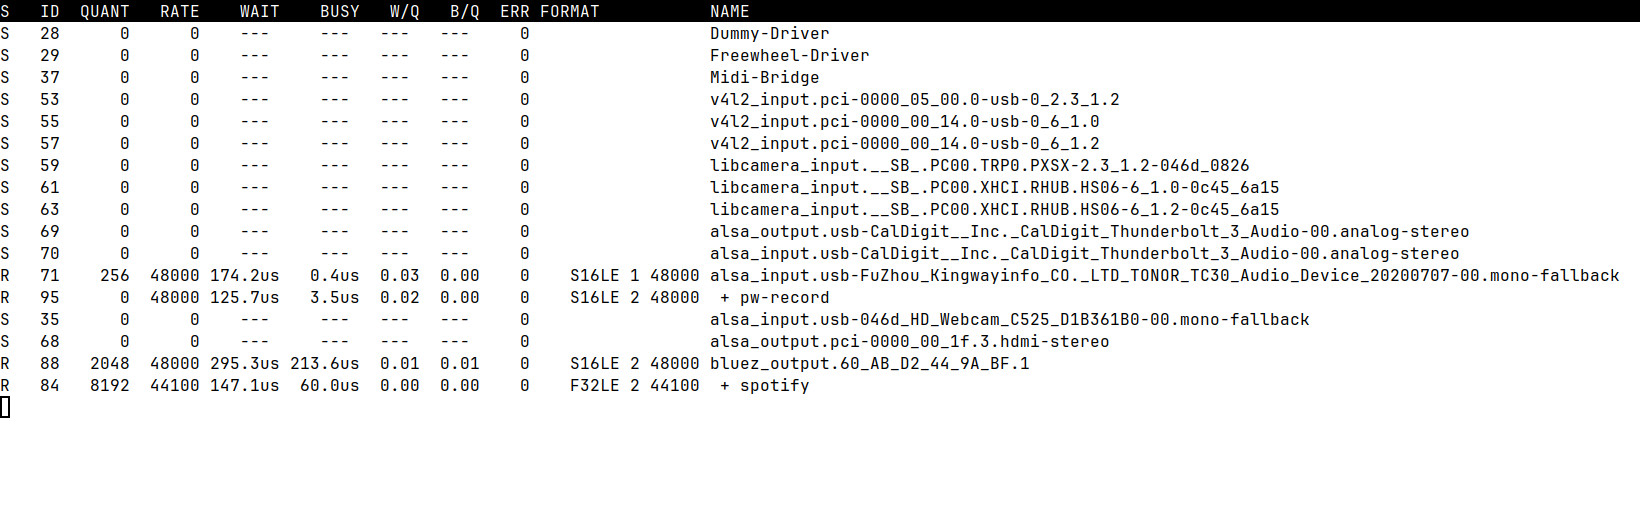
\includegraphics[height=0.5\textheight]{slides/audio-pipewire/pw-top.jpg}\\
  \end{center}
\end{frame}



\begin{frame}{Tools rundown — \code{pw-profiler}}
  \begin{itemize}

  \item Allows profiling of all running nodes: it records many time
    durations while running then generates graphs once the command is
    stopped.

  \item Here is an example with a single \code{pw-play} node, first
    started with \code{PIPEWIRE_CONFIG_NAME} equal to
    \code{client.conf} then with \code{client-rt.conf} on a loaded
    system.

  \end{itemize}

  \begin{center}
    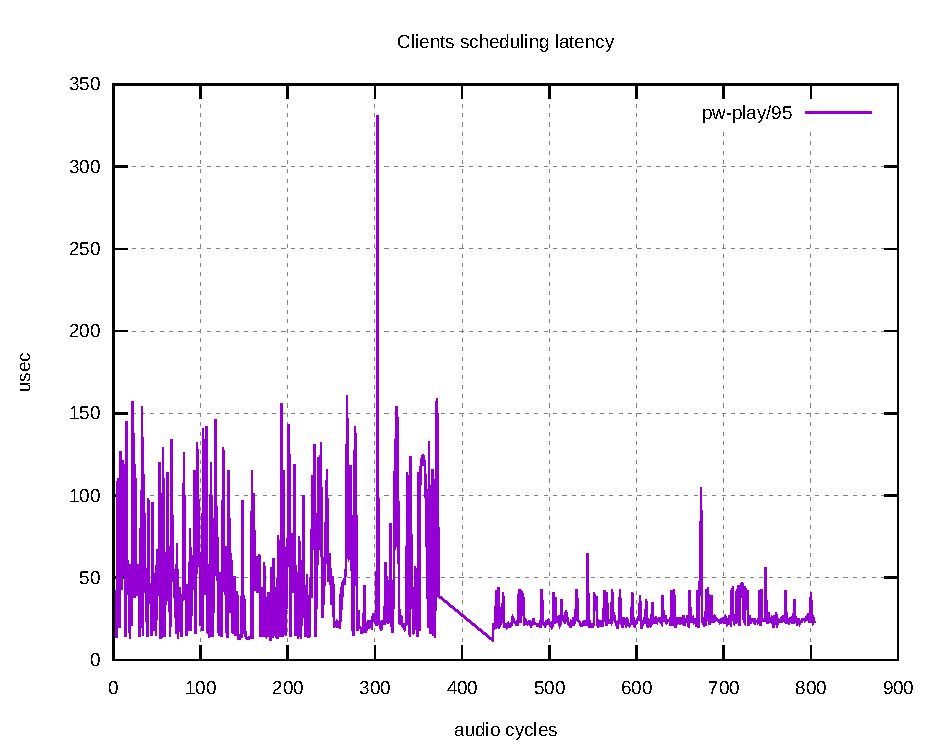
\includegraphics[height=0.5\textheight]{slides/audio-pipewire/pw-profiler-scheduling.pdf}
    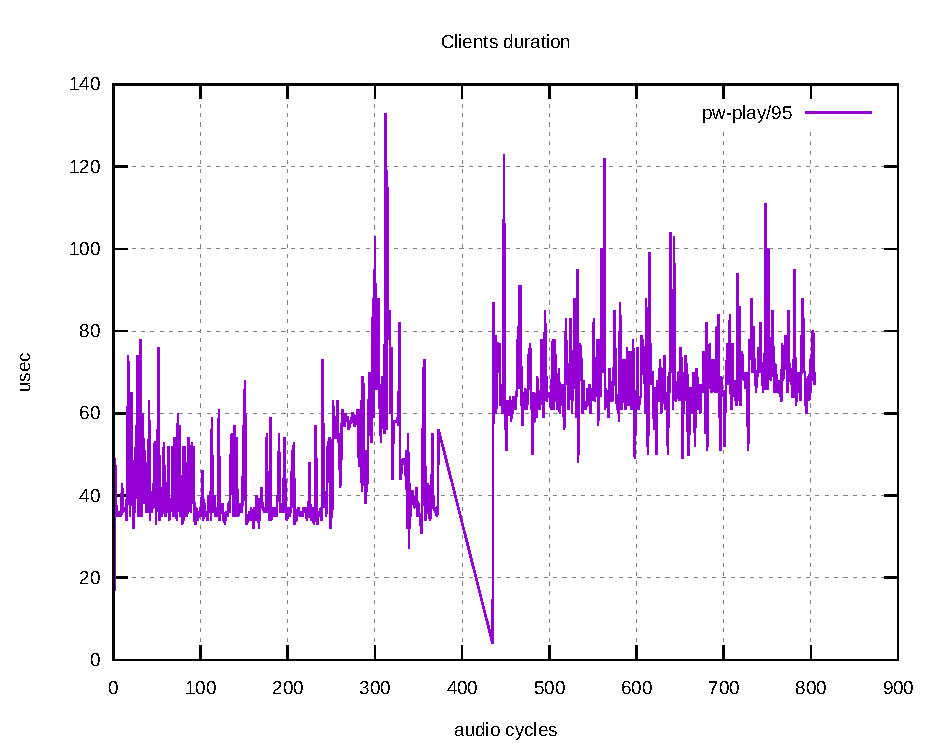
\includegraphics[height=0.5\textheight]{slides/audio-pipewire/pw-profiler-exectime.pdf}
  \end{center}
\end{frame}



\begin{frame}{Tools rundown — \code{pw-dot}}
  \begin{itemize}

  \item \code{pw-dot} creates a file named \code{pw.dot} which is a
    \href{https://graphviz.org/}{Graphviz} textual graph description
    file (\href{
    https://en.wikipedia.org/wiki/DOT_(graph_description_language)}{DOT}).

  \item By default, it connects to the PipeWire daemon and creates a
    graph representation of the global objects. It can also work from
    the output of \code{pw-dump} using the \code{--json} flag.

  \item That file can be turned into a graphical representation and
    viewed on a host using:\\\code{dot -Tsvg pw.dot > pw.svg && xdg-open pw.svg}

  \end{itemize}
\end{frame}



\begin{frame}{Tools rundown — \code{pw-cat}}
  \begin{itemize}

  \item Aliased to \code{pw-play}, \code{pw-record} and others, it is a
    simple tool to play or record media files.

  \item It uses \href{https://libsndfile.github.io/libsndfile/
    }{libsndfile} for a large audio format support.

  \item It has many options available to control the exposed props and
    params:

    \begin{itemize}
    \item \code{--target} allows asking to be routed to a given node;
    \item \code{--latency} asks for a given latency (therefore buffer size);
    \item \code{--quality} controls the adaptive resampling;
    \item \code{--rate}, \code{--channels}, \code{--channel-map},
      \code{--format}, \code{--volume} are self-describing.
    \item etc.
    \end{itemize}

  \end{itemize}
\end{frame}



\begin{frame}{Tools rundown — and a few others}
  \begin{itemize}

  \item \code{pw-link}: it allows listing, creating and deleting links.

  \item \code{pw-mon}: it monitors and dumps various events: it prints
    when a global object is added or removed, displays information
    relative to the \code{Core}, etc.

  \item \code{pw-loopback}: it creates two nodes that act as a virtual
    loopback.

  \item \code{pw-metadata}: it allows editing metadata, which are
    runtime-writable settings stored by the daemon. The allowed rates
    and quantum can be controlled at runtime using that method.

  \end{itemize}
\end{frame}



\begin{frame}{Tools rundown — \code{helvum} (1)}
  \begin{itemize}

  \item \href{https://gitlab.freedesktop.org/pipewire/helvum}{Helvum}
    is a real-time 2D patchbay.

  \item It gives an overview of the graph with the existing nodes and
    their ports. It also can create and delete links, allowing manual
    editing of the graph.

  \end{itemize}

  \begin{center}
    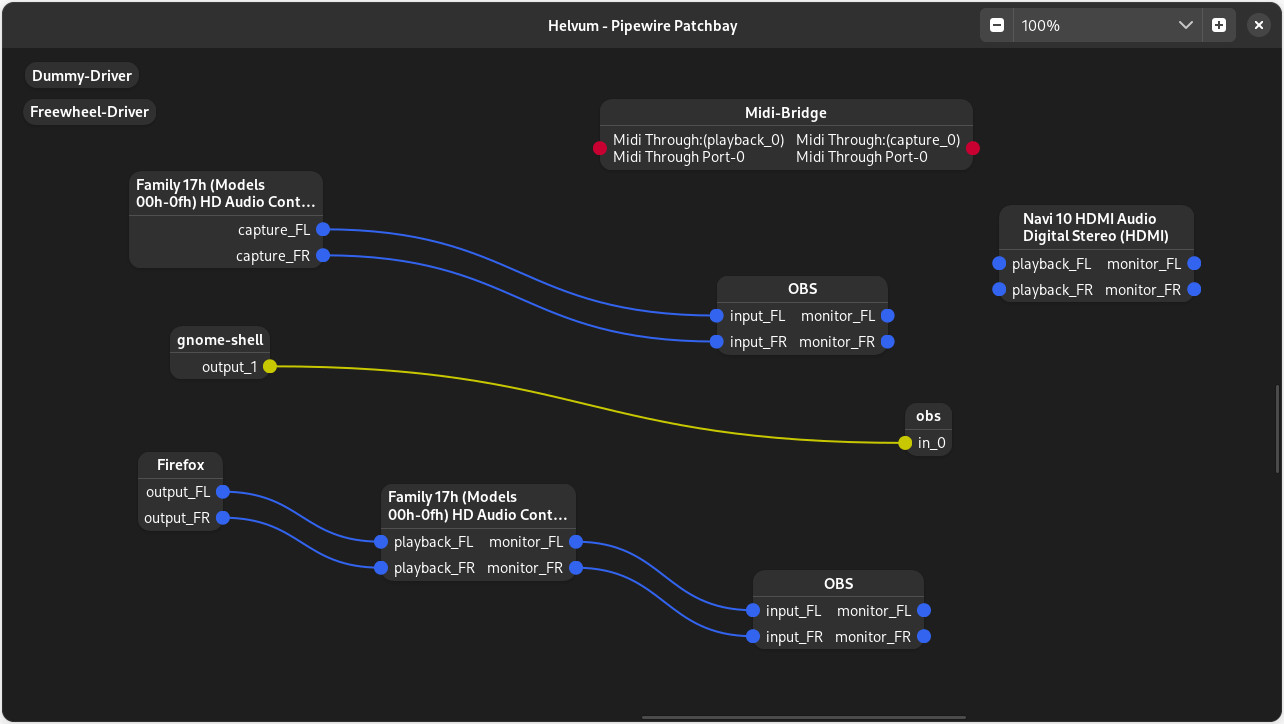
\includegraphics[height=0.5\textheight]{slides/audio-pipewire/helvum.jpg}
  \end{center}
\end{frame}



\begin{frame}{Tools rundown — \code{helvum} (2)}
  \begin{itemize}

  \item Helvum is a GUI software. We can however run it on our host and
    monitor our target if we have networking on the target.

  \item We use \href{http://www.dest-unreach.org/socat/}{socat} on the
    target to bridge the Unix socket from our target daemon over
    TCP/IP. We then use socat on the host to bridge the TCP/IP to a
    Unix socket that we will use as our PipeWire Unix socket for
    Helvum.

  \end{itemize}

  \begin{center}
    \includegraphics[height=0.3\textheight]{slides/audio-pipewire/helvum-target.pdf}
  \end{center}

\end{frame}



\begin{frame}[fragile]{Tools rundown — \code{helvum} (3)}
  \begin{columns}

    \column{0.9\textwidth}
    \begin{block}{}
      \fontsize{9}{9}\selectfont
        \begin{minted}{text}
# We run socat on the target, creating a redirection from the Unix
# socket /run/pipewire-0 to a TCP/IP server on port 8000.
ssh $login@$ip "socat TCP4-LISTEN:8000 UNIX-CONNECT:/run/pipewire-0" &

# We run socat on the host, creating the redirection from the TCP/IP
# port 8000 on the target to the Unix socket /tmp/pipewire-0 on the
# host.
socat UNIX-LISTEN:/tmp/pipewire-0 TCP4:$ip:8000 &

# And we connect on the redirected Unix socket.
PIPEWIRE_RUNTIME_DIR=/tmp helvum
        \end{minted}
      \end{block}

  \end{columns}
\end{frame}



\subsection{Demo 1 — running PipeWire}



\begin{frame}{Demo 1 — introduction}
  \begin{itemize}

  \item Demo time!

  \item We will play audio to an \code{alsa-lib} device from an audio
    file.

  \item We will let our session manager discover ALSA devices and
    connect an output node to the ALSA sink node.

  \item The steps will be:

    \begin{enumerate}
    \item Start a PipeWire daemon;
    \item Start a WirePlumber daemon;
    \item Start a \code{pw-play} client;
    \item Study the graph status using various tools (\code{pw-dot},
      \code{pw-top}, \code{pw-cli}, etc).
    \end{enumerate}

  \end{itemize}
\end{frame}



\begin{frame}[fragile]{Demo 1 — pointers}
  \begin{enumerate}

  \item Start a PipeWire daemon.

    \begin{itemize}
    \item Running \code{pipewire} without arguments will start a client
      using \code{pipewire.conf}, which by default runs in daemon mode.
    \item At this state, the graph is rather empty. Objects are mostly
      modules and factories attached to the core client, and the
      client objects.
    \end{itemize}

  \item Start a WirePlumber daemon.
    \begin{itemize}
    \item It also picks its config automatically, no arguments required.
    \item Once started, we can notice that ALSA devices and attached
      nodes are created in the graph.
    \item Its log level is controlled using \code{WIREPLUMBER_DEBUG}.
    \end{itemize}

  \item Start a \code{pw-play} client;

    \begin{itemize}
    \item \code{pw-play <file>}
    \end{itemize}

  \item Study the graph status using various tools (\code{pw-dot},
      \code{pw-top}, \code{pw-cli}, etc).

  \end{enumerate}
\end{frame}



\subsection{Demo 2 — PipeWire filter-chains}



\begin{frame}{Demo 2 — introduction}
  \begin{itemize}

  \item We will keep our previous setup, but add a client that does
    equalization on the samples.

  \item The steps will be:

    \begin{enumerate}
    \item To create a new configuration file, for the client hosting the effect;
    \item Start a client using this config;
    \item Update links manually to make \code{pw-play} be routed to the
      effect, then to the ALSA sink node.
    \end{enumerate}

  \end{itemize}
\end{frame}



\begin{frame}[fragile]{Demo 2 — pointers}
  \begin{enumerate}

  \item To create a new configuration file, for the client hosting the effect.

    \begin{itemize}
    \item Recent PipeWire versions have a \code{filter-chain.conf}
      example with snippets for various needs (LADSPA with RNNoise,
      builtin effects, etc.).
    \item When modules spawn objects, they often give their own
      properties to children, and take arguments to set specific
      properties for each node. See \code{capture.props} and
      \code{playback.props}.
    \end{itemize}

  \item Start a client using this config.

    \begin{itemize}
    \item \code{pipewire -c filter-chain.conf}
    \end{itemize}

  \item Update links manually to make \code{pw-play} be routed to the
    effect, then to the ALSA sink node.

    \begin{itemize}
    \item This can be done using Helvum with its GUI.
    \item Otherwise,
      \code{pw-dot} or \code{pw-link --links} to get an overview then
      \code{pw-link <output-port> <input-port>} to create a new link.
    \end{itemize}

  \end{enumerate}
\end{frame}



\subsection{WirePlumber}



\begin{frame}{WirePlumber — session manager concept}
  \begin{itemize}

  \item \textbf{PipeWire} handles the processing of the media graph.

  \item An additional layer is required to implement the desired
    configuration of devices and the connections between nodes. That is
    implemented by the \textbf{session \& policy manager}.

  \item Two known open-source implementations exist:

    \begin{itemize}
    \item \href{https://gitlab.freedesktop.org/pipewire/media-session
      }{pipewire-media-session}: the initial implementation, deprecated;
    \item \href{https://pipewire.pages.freedesktop.org/wireplumber/
      }{WirePlumber}: recommended implementation.
    \end{itemize}

  \item \textbf{WirePlumber}
    implements a modular approach: it provides a high-level API and
    exposes it to \href{https://www.lua.org/}{Lua} scripts. Those
    implement the management logic.

  \item Technical stack: C, GLib (GObject), Lua engine, Meson \& Ninja.

  \item \href{https://pipewire.pages.freedesktop.org/wireplumber/}{Documentation}.

  \end{itemize}
\end{frame}



\begin{frame}{WirePlumber — default behavior}
  \begin{itemize}

  \item \textbf{WirePlumber} has a default behavior that tries to
    replicate the PulseAudio behavior, i.e. a desktop setup.

  \item It enumerates and adds \code{Device} objects for ALSA, BlueZ
    and others. It also puts those devices into a best-guess profile.

  \item Those devices get their associated nodes created automatically.

  \item Audio routing is based on two default nodes:

    \begin{itemize}
    \item An \code{Audio/Sink} node is for applications that want to
      emit audio. All \code{Output/Audio} nodes get routed to it.
    \item An \code{Audio/Source} node is for applications that require a
      microphone input. All \code{Input/Audio} nodes get routed to it.
    \end{itemize}

  \item Nodes can also request to be routed to:

    \begin{enumerate}
    \item a target node using \code{target.object};
    \item nothing automatically using \code{node.autoconnect}.
      WirePlumber will not create any automatic link, letting any
      PipeWire client create the desired links.
    \end{enumerate}

  \end{itemize}
\end{frame}



\begin{frame}{WirePlumber — configuration (1)}
  \begin{itemize}

  % TODO: update once JSON config gets released (ie WP version 0.5)

  \item The config lookup logic is the same as PipeWire's.

  \item Lua files are being run when starting. They return
    which \textbf{WirePlumber modules} and \textbf{scripts} must be run
    at runtime, with the argument to be passed to them (as Lua tables).

  \item By default, there are three config: \code{bluetooth.lua},
    \code{main.lua} \& \code{policy.lua}.

  \end{itemize}
\end{frame}



\begin{frame}{WirePlumber — configuration (2)}
  \begin{itemize}

  \item Let's take the \code{main.lua} section, and focus on the
    ALSA-focused files:

    \begin{itemize}
    \item \code{00-functions.lua}: declares helper functions
      \code{load_module}, \code{load_script}, etc.
    \item \code{30-alsa-monitor.lua}: declares two config tables
      \code{alsa_monitor.properties} \& \code{alsa_monitor.rules} and a
      function \code{alsa_monitor.enable()}.
    \item \code{50-alsa-config.lua}: edits \code{.properties}
      \& \code{.rules} to the desired config.
    \item \code{90-enable-all.lua}: calls \code{.enable()}.
    \end{itemize}

  \item The \code{.enable()} function is what loads the right modules
    and scripts for ALSA support. It is done at the end because it
    requires \code{.properties} and \code{.rules} to be modified
    beforehands.

  \item \code{.properties} has ALSA support config: it can toggle D-Bus
    device reservation, toggle MIDI support, etc.

  \item \code{.rules} defines properties that should be applied to ALSA
    devices or nodes and conditions for applying those.

  \end{itemize}
\end{frame}



\begin{frame}[fragile]{WirePlumber — configuration (3)}
  \begin{itemize}
  \item Example disabling dependency on the D-Bus session instance:
  \end{itemize}

    \begin{block}{}
      \fontsize{11}{11}\selectfont
        \begin{minted}{lua}
-- /etc/wireplumber/main.lua.d/55-disable-dbus-features.lua
alsa_monitor.properties["alsa.reserve"] = false
default_access.properties["enable-flatpak-portal"] = false
          \end{minted}
        \end{block}

  \begin{itemize}
  \item Example disabling persistent storage (for read-only filesystems):
  \end{itemize}

    \begin{block}{}
      \fontsize{11}{11}\selectfont
        \begin{minted}{lua}
-- /etc/wireplumber/main.lua.d/60-disable-persistent-state.lua
device_defaults.properties["use-persistent-storage"] = false
          \end{minted}
        \end{block}

\end{frame}



\begin{frame}[fragile]{WirePlumber — configuration (4)}

  \begin{itemize}
  \item Example adding a nickname:
  \end{itemize}

    \begin{block}{}
      \fontsize{10.5}{10.5}\selectfont
        \begin{minted}{lua}
-- /etc/wireplumber/main.lua.d/55-add-nick.lua
table.insert(alsa_monitor.rules, {
  matches = {
    { -- Exact card name, see `pw-cli ls Device` then `pw-cli info <id>`.
      -- This rule will apply to nodes associated with the device as
      -- well as nodes have this prop.
      { "api.alsa.card.name", "=", "foo" },
    }
  },
  apply_properties = { ["device.nick"] = "bar" },
})
        \end{minted}
      \end{block}

\end{frame}



\begin{frame}{WirePlumber — permission handling (1)}
  \begin{itemize}

  \item Another task of the session \& policy manager is \textbf{permission
    management}.

  \item That is handled, in PipeWire >= 0.3.83, using two PipeWire daemon sockets:

    \begin{itemize}
    \item Clients joining \code{pipewire-0-manager} have full permissions, seen
      using property \code{pipewire.access = "unrestricted"}.
    \item Client joining \code{pipewire-0} must be given permissions by the
      session manager, i.e. WirePlumber. Propery \code{pipewire.access} is
      \code{"default"}.
    \end{itemize}

  \item Permissions can be granted on a per-object-basis for each client. Else
    each client has a default permission assigned to it.

  \end{itemize}
\end{frame}



\begin{frame}{WirePlumber — permission handling (2)}
  \begin{itemize}
  \item Example restricting

  \item Another task of the session \& policy manager is \textbf{permission
    management}.

  \item That is handled, in PipeWire >= 0.3.83, using two PipeWire daemon sockets:

    \begin{itemize}
    \item Clients joining \code{pipewire-0-manager} have full permissions.
    \item Client joining \code{pipewire-0} must be given permissions by the
      session manager, i.e. WirePlumber.
    \end{itemize}

  \item Permissions can be granted on a per-object-basis for each client. Else
    each client has a default permission assigned to it.

  \end{itemize}
\end{frame}



% TODO: should we add info on scripts? Maybe give some examples?
%  - It might help clarify the diff between config and scripts.
%  - It might help getting started on writing basic logic.
%  - It could help unmistify what WP does, and that people can do it
%    manually if they don't need a session manager.

% TODO: might want to mention stuff that requires RW FS.


\subsection{Demo 3 — interacting with WirePlumber}



\begin{frame}{WirePlumber — demo time! (1)}
  \begin{itemize}

  \item We'll use our previous setup, focusing on WirePlumber abilities.

  \item The steps will be:

    \begin{enumerate}
    \item Start PipeWire and WirePlumber;
    \item Target a specific node;
    \item Modify the default playback node, setting it to our filter-chain;
    \item Have a look at device profiles.
    \end{enumerate}

  \end{itemize}
\end{frame}



\begin{frame}{WirePlumber — demo time! (2)}
  \begin{enumerate}

  \item Start PipeWire and WirePlumber.

    \begin{itemize}
    \item See demo 1 for explainations.
    \end{itemize}

  \item Target a specific node.

    \begin{itemize}
    \item This is done by nodes using \code{target.object} (previously
      \code{node.target}).
    \item It can be a node ID, node name or object path (see
      WirePlumber scripts for the logic).
    \item A node's properties are controlled when spawning it, so by
      its config or by its client (WirePlumber for example).
    \end{itemize}

  \item Modify the default playback node, setting it to our filter-chain.

    \begin{itemize}
    \item \code{wpctl set-default <id>} controls this.
    \item Nodes must have \code{media.class} equal to \code{Audio/Sink}
      (or similar) to appear in this list.
    \end{itemize}

  \item Have a look at device profiles.

    \begin{itemize}
    \item Those are params on the device objects. See \code{EnumProfile}
      and \code{Profile}.
    \end{itemize}

  \end{enumerate}
\end{frame}



\subsection{C API}



\begin{frame}[fragile]{C API — introduction}
  \begin{itemize}

  \item \code{libpipewire}: reference implementation, and currently the only one.

  \item Allows connecting to the daemon as a client.

  \item Rust bindings: \href{
    https://gitlab.freedesktop.org/pipewire/pipewire-rs}{pipewire-rs}.

  \item See \code{pkg-config} for CFLAGS and LDFLAGS:

    \begin{minted}{text}
$ pkg-config --cflags --libs libpipewire-0.3
    \end{minted}

  \item To initialise the library (logging, randomness, etc.), call:
    \begin{minted}{c}
void pw_init(int *argc, char **argv[]);
    \end{minted}

  \end{itemize}
\end{frame}



\begin{frame}[fragile]{C API — SPA}
  \begin{itemize}

  \item A building block is worth mentioning, \textbf{Simple Plugin
    API} (SPA). It contains the following:

    \begin{itemize}
    \item A \href{https://docs.pipewire.org/page_spa.html#autotoc_md225
      }{plugin format} encapsulating shared objects, allowing
      runtime introspection of the plugin content.
    \item A Type-Length-Value data container called \href{
      https://docs.pipewire.org/page_spa_pod.html}{POD}. It is
      header-only, with support for basic types (int, float,
      string, etc.) and nested types (array, struct, objects).
    \item \href{https://docs.pipewire.org/group__spa__utils.html}{Utility
      functions} as header-only: string handling utilities,
      relaxed JSON parsing (used for config files), a ringbuffer
      implementation, etc.
    \item \href{https://docs.pipewire.org/group__spa__support.html}{Support
      interfaces} provided by the system, with multiple
      possible implementations: logging, file-descriptor polling, etc.
    \end{itemize}

  \item Platform resources (ALSA, bluez5, vulkan, etc.) are exposed
    as SPA plugins and used internally by PipeWire or WirePlumber.

  \end{itemize}
\end{frame}



\begin{frame}[fragile]{C API — event-loop}
  \begin{itemize}
  \item At the core of each client: an \code{epoll(2)}-based event-loop
    is running.
  \item \code{pw_main_loop} is a wrapper around \code{pw_loop}
    providing a simple-to-use API.
  \end{itemize}

      \begin{block}{}
        \fontsize{9}{9}\selectfont
          \begin{minted}{c}
/** Create a new main loop. */
struct pw_main_loop *
pw_main_loop_new(const struct spa_dict *props);

/** Get the loop implementation */
struct pw_loop * pw_main_loop_get_loop(struct pw_main_loop *loop);

/** Destroy a loop */
void pw_main_loop_destroy(struct pw_main_loop *loop);

/** Run a main loop. This blocks until \ref pw_main_loop_quit is called */
int pw_main_loop_run(struct pw_main_loop *loop);

/** Quit a main loop */
int pw_main_loop_quit(struct pw_main_loop *loop);
          \end{minted}
      \end{block}
\end{frame}



\begin{frame}[fragile]{C API — context}
  \begin{itemize}

  \item A \code{pw_context} instance is at the heart of the C API. It
    allows connection to the daemon and it manages locally available
    ressources.

  \item It does the following:

    \begin{itemize}
    \item Parsing of the appropriate configuration.
    \item Start of the processing thread \& associated data loop.
    \item Handling of local ressources: memory pool, work queue,
      \textbf{proxies}, local modules
    \end{itemize}

  \end{itemize}

      \begin{block}{}
        \fontsize{9}{9}\selectfont
          \begin{minted}{c}
/** Make a new context object for a given main_loop */
struct pw_context * pw_context_new(struct pw_loop *main_loop,
                struct pw_properties *props, size_t user_data_size);

/** Connect to a PipeWire instance */
struct pw_core * pw_context_connect(struct pw_context *context,
                struct pw_properties *properties, size_t user_data_size);
          \end{minted}
      \end{block}
\end{frame}



\begin{frame}{C API — proxies}
  \begin{itemize}

  \item Think as \textbf{proxies} as file descriptors for PipeWire
    objects. They are local references to global PipeWire objects.

  \item The equivalent on the daemon side are called \textbf{resources}.

  \item A client starts with two proxies:

    \begin{enumerate}
    \item One pointing to the \code{Core} object.
    \item Another one to the global \code{Client} object that represents
      itself.
    \end{enumerate}

  \end{itemize}
\end{frame}



\begin{frame}[fragile]{C API — registry}
  \begin{itemize}

  \item The PipeWire daemon handles a list of objects. Those are
    known as \textbf{global} objects and are represented by
    \code{pw_global} structures.

  \item \code{pw_registry} is a singleton structure that allows clients
    to track existing globals. It works by registering a callback to be
    called on new global object events.

  \end{itemize}

      \begin{block}{}
        \fontsize{9}{9}\selectfont
          \begin{minted}{c}
struct pw_registry_events {
#define PW_VERSION_REGISTRY_EVENTS  0
        uint32_t version;
        void (*global) (void *data, uint32_t id, uint32_t permissions,
                const char *type, uint32_t version,
                const struct spa_dict *props);
        void (*global_remove) (void *data, uint32_t id);
};

struct pw_registry * pw_core_get_registry(struct pw_core *core,
        uint32_t version, size_t user_data_size);

void pw_registry_add_listener(struct pw_registry *registry,
        struct spa_hook *hook, struct pw_registry_events *events,
        void *data);
          \end{minted}
      \end{block}
\end{frame}



\begin{frame}[fragile]{C API — example 1, monitoring global objects}
  \begin{block}{}
    \fontsize{8}{8}\selectfont
      \begin{minted}{c}
/* We will run indefinitely, getting events for each added and removed global
 * object.
 *
 * An influx of Registry::Global events will come in at the start to list all
 * already-existing globals. Use the Core::Sync method and Core::Done event to
 * know when that initial sync is done. See pw_core_sync(). */
#include <pipewire/pipewire.h>

static void registry_event_global(void *data, uint32_t id, uint32_t permissions,
                const char *type, uint32_t version, const struct spa_dict *props) {
        printf("object added: id:%u\ttype:%s/%d\n", id, type, version);
}

static void registry_event_global_remove(void *data, uint32_t id) {
        printf("object removed: id:%u\n", id);
}

static const struct pw_registry_events registry_events = {
        PW_VERSION_REGISTRY_EVENTS,
        .global = registry_event_global,
        .global_remove = registry_event_global_remove,
};
    \end{minted}
  \end{block}
\end{frame}



\begin{frame}[fragile]{C API — example 1, monitoring global objects}
  \begin{block}{}
    \fontsize{8}{8}\selectfont
      \begin{minted}{c}
int main(int argc, char **argv) {
  pw_init(&argc, &argv);

  struct pw_main_loop *loop = pw_main_loop_new(NULL);
  struct pw_context *context = pw_context_new(pw_main_loop_get_loop(loop), NULL, 0);
  struct pw_core *core = pw_context_connect(context, NULL, 0);
  struct pw_registry *registry = pw_core_get_registry(core, PW_VERSION_REGISTRY, 0);

  struct spa_hook registry_listener;
  spa_zero(registry_listener);
  pw_registry_add_listener(registry, &registry_listener, &registry_events, NULL);

  pw_main_loop_run(loop);

  pw_proxy_destroy((struct pw_proxy*)registry);
  pw_core_disconnect(core);
  pw_context_destroy(context);
  pw_main_loop_destroy(loop);

  return 0;
}
    \end{minted}
  \end{block}
\end{frame}



\begin{frame}{C API — node implementations}
  \begin{itemize}

  \item Implementing a raw node is not straight-forward, requiring to
    implement many book-keeping methods (see \code{struct spa_node_methods}).

  \item PipeWire provides two abstractions for implementing nodes:

    \begin{itemize}

    \item \code{pw_filter}: DSP-type work, works on raw \code{f32}
      samples, without additional buffering.

    \item \code{pw_stream}: more high level, it provides the following
      features:
      \begin{itemize}
      \item \textbf{Buffering:} a stream can emit more samples than
        the current cycle quantum and those will be buffered.
      \item \textbf{Format negociation:} the client can expose multiple
        supported formats and negociation will occur when changing from
        idle to running.
      \item \textbf{Format conversion:} sample type, planar/interleaved,
        channel mapping, rate resampling.
      \end{itemize}

    \end{itemize}

  \item See example implementations of source nodes:
    \begin{itemize}
    \item Filter: \code{src/examples/audio-dsp-src.c}
    \item Stream: \code{src/examples/audio-src.c}
    \end{itemize}

  \end{itemize}
\end{frame}



\begin{frame}[fragile]{C API — \code{pw_filter} process event}
  \begin{columns}
    \column{0.8\textwidth}
      \begin{block}{}
        \fontsize{8}{8}\selectfont
          \begin{minted}{c}
static void on_process(void *userdata, struct spa_io_position *position) {
  struct data *data = userdata;
  double *acc = data->out_port->accumulator;
  uint64_t n_samples = position->clock.duration;

  /* Fetch the sample buffer. The first argument is the port user data
   * (as returned by pw_filter_add_port), it is used to identify our
   * port (think container_of). */
  float *out = pw_filter_get_dsp_buffer(data->out_port, n_samples);
  if (out == NULL)
    return;

  for (uint64_t i = 0; i < n_samples; i++) {
    *acc += 2 * M_PI * 440 / 44100;   /* Grow our accumulator */
    *acc = remainder(*acc, 2 * M_PI); /* Avoid overflows */
    *out++ = sin(*acc) * 0.7;         /* Compute a sample */
  }
}

static const struct pw_filter_events filter_events = {
  PW_VERSION_FILTER_EVENTS,
  .process = on_process,
};
          \end{minted}
        \end{block}
  \end{columns}
\end{frame}



\begin{frame}[fragile]{C API — \code{pw_stream} process event}
  \begin{columns}
    \column{0.5\textwidth}
      \begin{block}{}
        \fontsize{8}{8}\selectfont
          \begin{minted}{c}
static void on_process(void *userdata) {
  struct data *data = userdata;

  struct pw_buffer *b = pw_stream_dequeue_buffer(
      data->stream);
  assert(b != NULL);

  struct spa_buffer *buf = b->buffer;
  uint8_t *p = buf->datas[0].data;
  assert(p != NULL);

  int stride = sizeof(float) * CHANNELS;
  int n_frames = SPA_MIN(b->requested,
      buf->datas[0].maxsize / stride);

  fill_f32(&data->accumulator, p, n_frames);

  buf->datas[0].chunk->offset = 0;
  buf->datas[0].chunk->stride = stride;
  buf->datas[0].chunk->size = n_frames * stride;

  pw_stream_queue_buffer(data->stream, b);
}
          \end{minted}
        \end{block}

    \column{0.5\textwidth}
      \begin{block}{}
        \fontsize{8}{8}\selectfont
          \begin{minted}{c}
#define CHANNELS 2
#define FREQ     440
#define RATE     44100

static void fill_f32(float *acc, float *dest,
    int n_frames) {
  for (int i = 0; i < n_frames; i++) {
    *acc += M_PI_M2 * FREQ / RATE;
    *acc = remainder(*acc, 2 * M_PI);

    float val = sin(*acc) * 0.7;
    for (int c = 0; c < CHANNELS; c++)
      *dst++ = val;
  }
}

static const
struct pw_stream_events stream_events = {
  PW_VERSION_STREAM_EVENTS,
  .process = on_process,
};
          \end{minted}
        \end{block}
  \end{columns}
\end{frame}



\subsection{Going further}



\begin{frame}{Going further}
  \begin{itemize}

  \item For MIDI support, see \code{pw-cat --midi}, \code{pw-mididump}
    and \href{https://docs.pipewire.org/page_midi.html}{the documentation}.

  \item For the PulseAudio compatibility layer, see
    \href{https://docs.pipewire.org/page_module_protocol_pulse.html
    }{module-protocol-pulse} and \href{
      https://docs.pipewire.org/page_pulseaudio.html}{this documentation page}.

  \item For the JACK compatibility layer, look at \code{pw-jack}.

  \item For video support, see many examples in \code{src/examples/}.

  \item For audio over IP, see modules \code{roc-*}, \code{pulse-tunnel},
    \code{netjack2-*}, \code{rtp-*}, \code{protocol-simple}, \code{avb}.

  \end{itemize}
\end{frame}
